Рассмотрим два компьютера, соединённых проводом. При такой связи необходимо доставлять биты в том же порядке, в котором они были отправлены передающей машиной. Для реализации подобной связи были созданы различные протоколы передачи данных. Часть таких протоколов в своей реализации использует разбиение сегментов данных на следующие 4 вида:

\begin{itemize}
	\item сегменты, которые были отосланы и имеют подтверждение от
	приемника
	\item сегменты, которые были отосланы и не имеют подтверждения от
	приемника
	\item сегменты, которые могут быть отосланы
	\item сегменты, которые не могут быть отосланы
\end{itemize}

Передавать сегменты всех типов в правильном порядке проблематично из-за возможных ошибок при передаче. Чтобы решить эту проблему, необходимо воспользоваться некоторым окном фиксированного размера, в рамках которого будет происходить доставка сегментов. Визуализация такого подхода представлена на рис. 1.

\begin{figure}[H]
	\begin{center}
		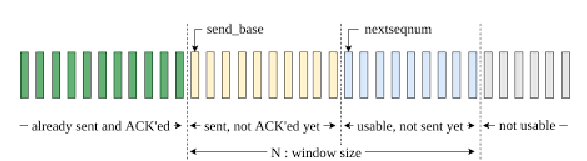
\includegraphics{im1}
		\caption{Визуализация передачи данных с использованием скользящего окна}
	\end{center}
\end{figure}

Идея заключается в том, чтобы выявлять и исправлять все ошибки передачи данных в рамках окна. После этого происходит его смещение к сегментам с большим порядковым номером и процедура передачи повторяется. Рассмотрим два протокола, использующих данный подход.

\subsection{Протокол Go-Back-N}

Особенностью протокола Go-Back-N является отправка всего набора сегментов, находящихся в рамках скользящего окна, не дожидаясь ответа от приемника. Таким образом, после заполнения окна отправленными, но не
подтвержденными сегментами, источник ожидает получения подтверждения
для всех сегментов. В случае, если один из сегментов не получил
подтверждения доставки за некоторое фиксированное время, называемое
также таймером, то источник повторяет отправку всех сегментов окна,
начиная с этого сегмента. Рассмотрим данный протокол на примере случая,
когда размер окна равен четырем (рис. 2).

\begin{figure}[H]
	\begin{center}
		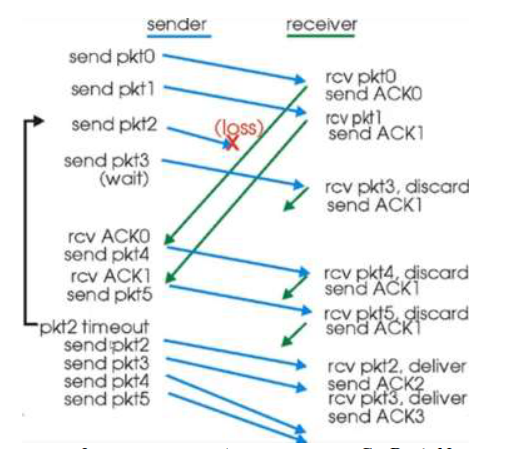
\includegraphics[scale=0.6]{im2}
		\caption{Диаграмма работы протокола Go-Back-N}
	\end{center}
\end{figure}

Источник начинает осуществлять посылку сегментов приемнику. Так как размер окна равен четырем, источник может послать четыре
сегмента, т.е. сегменты с номерами 0, 1, 2, 3, без получения подтверждения, после чего источник должен ожидать подтверждения. В указанном примере сегмент номер 2 был потерян при передаче. В связи
с этим сегменты 3, 4, 5 поступили вне очереди, поэтому они не должны быть подтверждены приемником.
По истечении срока ожидания подтверждения отправитель заново посылает приёмнику весь пул сегментов.

\subsection{Протокол Selective Repeat}

Протокол Go-Back-N затрачивает довольно много избыточных ресурсов, посылая подтверждённые данные по несколько раз в случае ошибок. В связи с этим, при больших размерах окна и низкой пропускной способности канала передачи становится ярко выраженной низкая эффективность данного протокола. Протокол Selective Repeat позволяет
избегать повторной передачи тех сегментов, которые безошибочно, но вне
очереди, были приняты приемником. Повторно передаются только сегменты,
переданные с ошибками.

Таким образом, для подтверждения повторно переданного сегмента
приемник должен послать источнику индивидуальное подтверждение, и
сегменты, пришедшие без ошибок, но вне очереди, должны быть
подтверждены. Так же, как и в протоколе Go-Back-N, в Selective Repeat окно размера N используется для ограничения количества посланных, но не
подтвержденных сегментов. Но в данном протоколе в окне могут находиться
посланные и подтвержденные сегменты. Рассмотрим работу протокола для
того же примера, когда размер окна равен четырем (рис. 3).

\begin{figure}[H]
	\begin{center}
		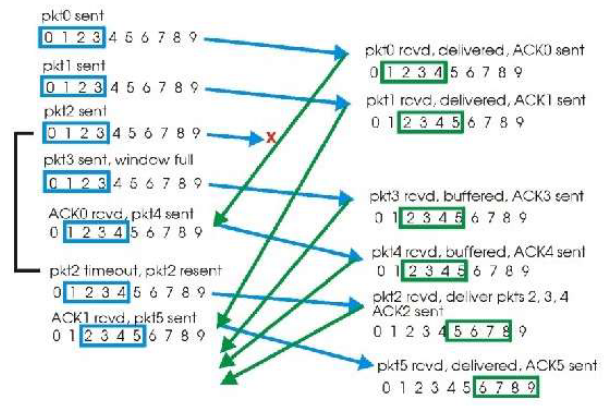
\includegraphics[scale=0.6]{im3}
		\caption{Диаграмма работы протокола Selective Repeat}
	\end{center}
\end{figure}

Как можно заметить, данный протокол является более выгодным при
наличии ошибок передачи с точки зрения объема пересылаемых данных, однако сдвиг окна выполняется в соответствии с более сложной логикой: данные должны быть переданы в заданном порядке, поэтому при сдвиге окна нельзя допускать перекрытия старого окна новым.
Для этого размер окна не должен превышать половины от количества
порядковых номеров.
